\documentclass[12pt]{article}

\usepackage{sbc-template}
\usepackage{graphicx,url}
\usepackage[utf8]{inputenc}
\usepackage[brazil]{babel}
\usepackage{amsmath}
\usepackage{listings}
\usepackage{xcolor}

% Configurações para exibição de código-fonte
\lstset{
    language=C++,
    basicstyle=\ttfamily\footnotesize,
    keywordstyle=\color{blue},
    stringstyle=\color{red},
    commentstyle=\color{gray},
    numbers=left,
    numberstyle=\tiny,
    stepnumber=1,
    breaklines=true,
    frame=single,
    captionpos=b
}

\sloppy

\title{Desenvolvimento de um Simulador de Relógio Digital e Alarme\\ utilizando Lógica Discreta em C++ e Verilog}

\author{Francisco Passos dos S. Alves\inst{1}, João Vitor V. Leão\inst{1}, \\ Karlos Danyel S. Gomes\inst{1}, Lucca Pedreira Dultra\inst{1}}

\address{Departamento de Computação -- Universidade Federal de Sergipe (UFS)\\
  São Cristóvão -- SE -- Brasil
  \email{\{francisco.alves, joao.leao2, karlos.gomes2, lucca.dultra\}@dcomp.ufs.br} 
}

\begin{document} 

\maketitle

\begin{abstract}
  This paper describes the development of a digital clock and alarm simulator, inspired by a hardware project from the WR Kits channel. To consolidate learning in Digital Systems, the primary focus of this work was modeling discrete CMOS chips (CD4000 series) in C++ using object-oriented principles, intricately replicating low-level hardware behavior. As a complementary validation step, a small portion of the logic was also prototyped in Verilog using Verilator.
\end{abstract}
     
\begin{resumo} 
  Este artigo descreve o desenvolvimento de um simulador de relógio digital e alarme, inspirado em um projeto de hardware do canal WR Kits. Para consolidar o aprendizado em Sistemas Digitais, o foco principal deste trabalho foi a modelagem de chips CMOS discretos (série CD4000) em C++ utilizando orientação a objetos, replicando minuciosamente o comportamento de hardware em baixo nível. Como etapa complementar de validação, uma pequena parcela da lógica também foi prototipada em Verilog utilizando Verilator.
\end{resumo}

\section{Introdução}

O estudo de Sistemas Digitais compreende a transição fundamental entre a abstração lógica booleana e a implementação física de circuitos eletrônicos. Um dos projetos mais clássicos para consolidar tais conhecimentos é o desenvolvimento de um relógio digital síncrono. 

Este trabalho propõe uma abordagem focada em software: a emulação rigorosa do hardware lógico por meio de programação. Inspirado no projeto físico \textit{RELÓGIO DIGITAL} do canal WR Kits, recriamos o comportamento de circuitos integrados (CIs) discretos, como contadores, decodificadores e flip-flops. O objetivo principal é emular o comportamento exato das portas lógicas, sinais de \textit{clock} e cascatas de contagem, utilizando a linguagem C++ para a construção estrutural do circuito. 

Para estender o escopo, como solicitado pelo professor, o grupo adicionou um sistema completo de alarme com memória e comparação de tempo e dias da semana, exigindo uma integração robusta entre lógica combinacional e sequencial.

\section{Fundamentação Teórica e Componentes}

A arquitetura do relógio e do alarme foi projetada com base no funcionamento de componentes discretos reais (em sua maioria da família CMOS CD4000). Na simulação em C++, cada chip foi implementado como uma classe independente, respeitando rigorosamente suas entradas, saídas e a dependência das bordas de \textit{clock}.

\begin{itemize}
    \item \textbf{CD4029 (Contador Up/Down):} Utilizado para a contagem dos minutos e horas. O \textit{ripple carry} foi modelado para que o contador subsequente só avance quando o anterior gerar \textit{Carry Out}.
    \item \textbf{CD4511 (Decodificador BCD para 7 Segmentos):} Converte a saída binária dos contadores para ativar os segmentos no \textit{display}.
    \item \textbf{CD4017 (Contador Johnson):} Empregado como indicador de meridiano (AM/PM) e para gerenciar os dias da semana no alarme.
    \item \textbf{CD4040 (Divisor de Frequência):} Permite gerar o pulso de 1 Hz para o relógio em tempo real, além de modos de ajuste rápido e lento.
    \item \textbf{CD4013 (Flip-Flop D) e CD4063 (Comparador):} Utilizados em conjunto no módulo de alarme para armazenar o horário programado e compará-lo com o barramento de tempo atual.
\end{itemize}

Para ilustrar a emulação de hardware em C++, a Listing \ref{lst:cd4017} demonstra a implementação do método de deslocamento (\textit{shift}) do CD4017, onde o estado interno só é alterado se o \textit{Clock Enable} permitir, emulando perfeitamente o limite de contagem e a saída ativa.

\begin{lstlisting}[caption={Emulação do comportamento de deslocamento do CI CD4017 em C++.}, label={lst:cd4017}]
void Chip4017::shift() {
    if (!ClockEnable){
        return;
    }
    value <<= 1;
    if (value >= (1u << LimitReset)) {
        value = 1;
    }
    outputs.fill(false);
    for (size_t i = 0; i < 10; i++) {
        outputs[i] = (value >> i) & 1;
    }
}
\end{lstlisting}

\section{Arquitetura e Implementação Lógica}

O projeto foi dividido em duas grandes estruturas de simulação interligadas via software: O \textit{Digital Clockwork} (módulo de tempo) e o \textit{Amazing Digital Alarm} (módulo de memória e disparo).

\subsection{O Relógio (Digital Clockwork)}

O funcionamento inicia-se com o gerador de \textit{clock} emulado por \textit{threads} no C++, atuando como um CI 555 astável. O sinal passa pelo divisor de frequência (CD4040) e a contagem é feita pelos CIs CD4029. 

Para lidar com os \textit{resets} assíncronos (como reiniciar as dezenas de minutos ao chegar em 6), utilizou-se a emulação de portas lógicas AND (CD4081). Quando a condição é atingida, um pulso é enviado aos pinos de \textit{Preset Enable} dos contadores. A Figura \ref{fig:counter} ilustra o diagrama esquemático dessa etapa.

\begin{figure}[htpb]
    \centering
    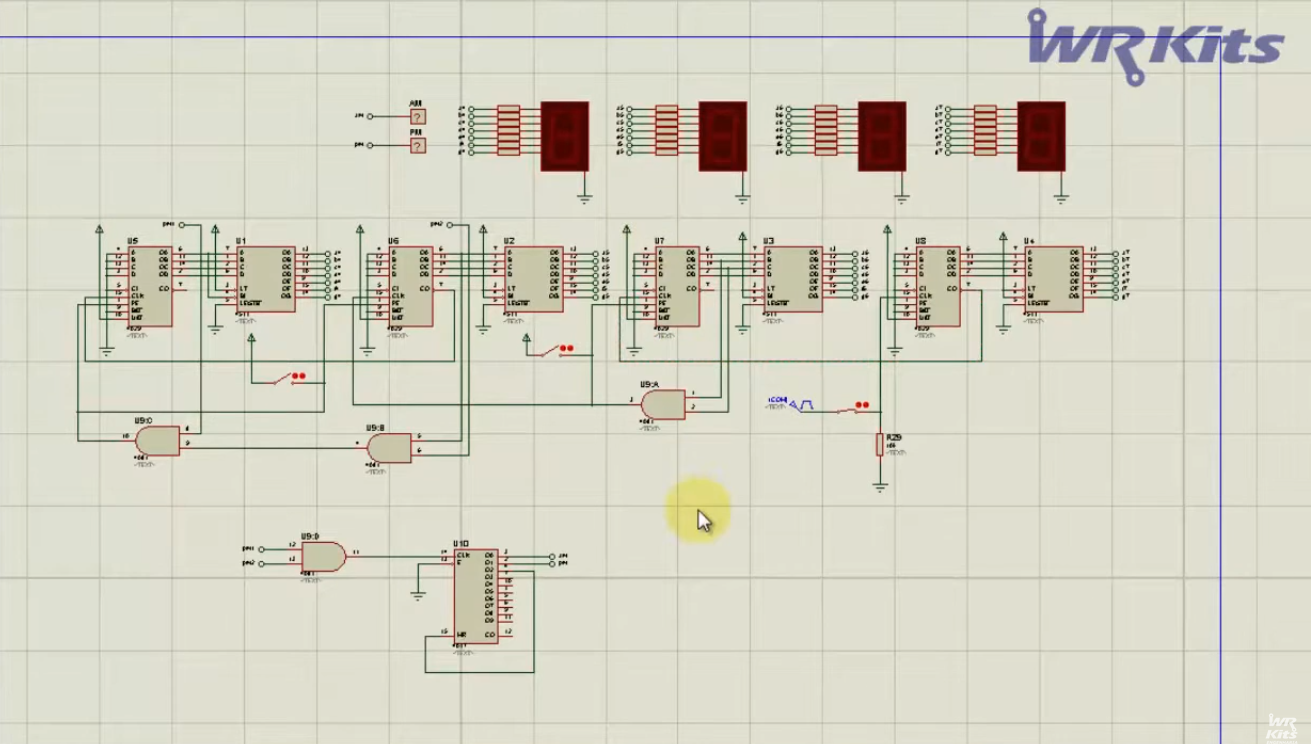
\includegraphics[width=0.8\textwidth]{counter.png}
    \caption{Diagrama esquemático do módulo de contagem do relógio digital.}
    \label{fig:counter}
\end{figure}

\subsection{O Alarme (Digital Alarm)}

O sistema de alarme consolida a lógica combinacional de magnitude. A inserção dos dias da semana ativos é feita por um arquivo \texttt{.week}, simulando chaves DIP físicas. A lógica interliga a validação do dia (portas AND/OR validando o CD4017) e a validação do tempo (cascata de comparadores CD4063 lendo a memória dos Flip-Flops CD4013). O esquema lógico projetado para o alarme pode ser visto na Figura \ref{fig:alarm}.

\begin{figure}[htpb]
    \centering
    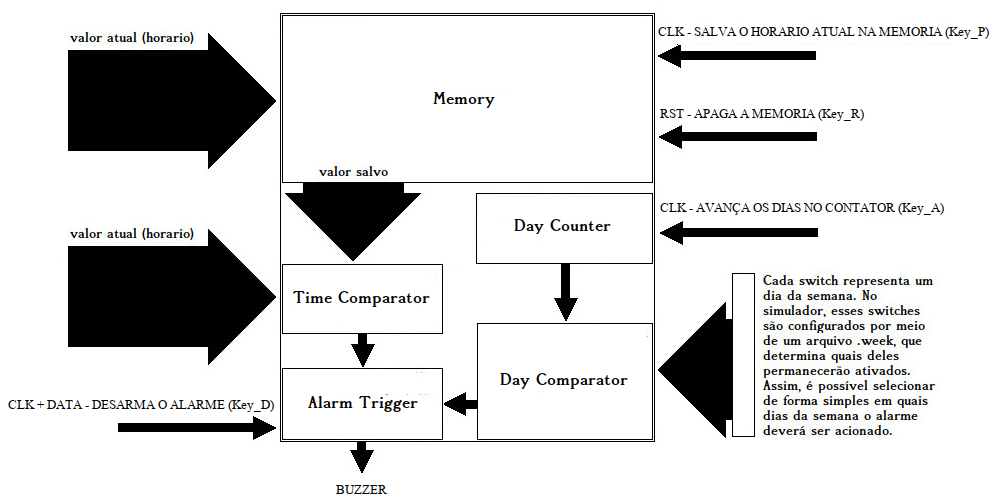
\includegraphics[width=0.9\textwidth]{project.png}
    \caption{Esquema lógico estrutural do sistema de alarme (\textit{Amazing Digital Alarm}).}
    \label{fig:alarm}
\end{figure}

\subsection{Interface e Execução}

Toda a lógica simulada em C++ reflete seu estado em tempo real no terminal do sistema operacional, capturando eventos de teclado nativos para acionar funções como ajuste rápido de hora, programação do alarme e reset do sistema. A Figura \ref{fig:simulator} demonstra o projeto em execução.

\begin{figure}[htpb]
    \centering
    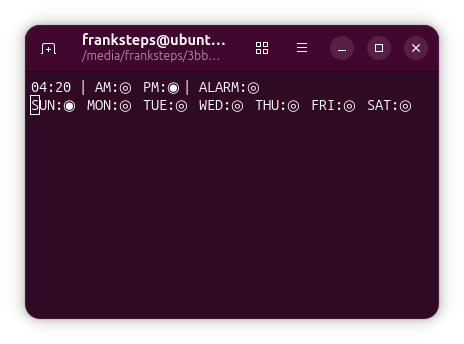
\includegraphics[width=0.7\textwidth]{simulator.png}
    \caption{Interface de execução do simulador renderizada no terminal.}
    \label{fig:simulator}
\end{figure}

\section{Validação Complementar em Verilog}

Embora o núcleo e o maior esforço do projeto residam na emulação de hardware orientada a objetos utilizando C++, realizou-se uma etapa complementar de prototipagem em linguagem de descrição de hardware (Verilog). 

Essa etapa menor teve como objetivo confirmar que a abstração lógica criada em software puro era sintetizável. O processo utilizou a ferramenta \textbf{Verilator}, convertendo o código Verilog em modelos C++ para permitir uma simulação mais proxima da implementação e validar a robustez da arquitetura desenhada.

\section{Conclusão}

O projeto atingiu com êxito o objetivo de consolidar os fundamentos de Sistemas Digitais. A recriação do hardware em C++, tratando os estados binários, \textbf{latches} e flancos de subida, exigiu uma compreensão profunda da folha de dados (\textbf{datasheet}) de cada circuito integrado utilizado. 

A expansão do sistema com o módulo de alarme forçou a utilização ostensiva de flip-flops para retenção de memória e comparadores de magnitude. O sucesso da simulação em C++ evidenciou que dominar a abstração de arquiteturas digitais permite transpor a lógica de circuitos físicos diretamente para sistemas de software complexos.

\begin{thebibliography}{9}

\bibitem[Rambo, 2015]{rambo:23} Rambo, W. (2015). \textit{Projeto de Relógio Digital com Lógica Discreta CMOS}. Canal WR Kits (YouTube).

\end{thebibliography}

\end{document}